\documentclass[]{article}

\usepackage{graphicx} %for å inkludere grafikk
\usepackage{verbatim} %for å inkludere filer med tegn LaTeX ikke liker
\usepackage{tabularx}
\usepackage{booktabs}
\usepackage{amsmath}
\usepackage{float}
\usepackage{color}
\usepackage{listings}
\usepackage{physics}
\usepackage{hyperref}
\usepackage{subfig}
\usepackage{mhchem}
\usepackage{natbib}
%opening
\title{}
\author{}

\begin{document}
	
\title{Fission: a TALYS report}
\author{Dorthea Gjestvang }
\date{December 2017}

\maketitle

\begin{abstract}

\end{abstract}

\section{Introduction}

Something about varying the fission barrier whitin the uncertainties, and then look at the (n,gamma) and (n,f) cross sections -> important for understanding how sensitive the system is to changes in the fission barrier

\section{Theory}
\subsection{Fission barrier}
When observing the average binding energy per nucleon, as seen in Figure \ref{fig:binding_energy_per_nucleon}, one can see that for $A \approx 60$ the binding energy per A peaks, and then starts to decrease for increasing A. For nuclei situated to the right of this peak, it is thus possible to release energy by splitting in two lighter fragments, that is to fission. However, when studying the chart of nuclei , one will observe that only a handfull of nuclei have spontaneous fission as their main decay mode, and they are generally heavy elements far from the valley of stability. This  is due to the so-called fission barrier. 
\par
\vspace{3mm}

\begin{figure}
	\centering
	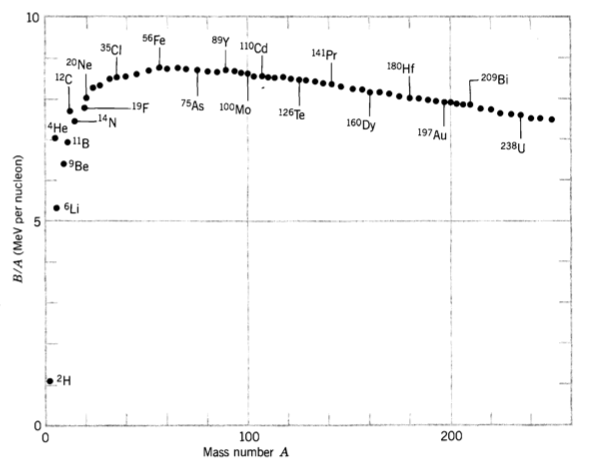
\includegraphics[scale=0.6]{binding_energy_per_nucleon.png}
	\caption{Average binding energy per nucleon. Figure from K.S. Krane p.67 \cite{Krane1988}}
	\label{fig:binding_energy_per_nucleon}
\end{figure}


 \noindent In the liquid model, the fission barrier is described as a smooth, parabolic barrier, and is shown in Figure \ref{fig:smooth_fission_barrier}. It describes the energy needed to separate the two fission fragments as a function of separation distance. The fission barrier is due to both the nuclear force and the Coloumb force. A picture on why there is a fission barrier, is that in order for the two would-be fission fragments to separate, they have to get out of the potential well that is the nuclear force, and then pass the Coloumb barrier surrounding the nucleus. Thus energy must be applied for the fragments to be able to separate. This energy needed is often referred to as the activation energy, and is shown in Figure \ref{fig:smooth_fission_barrier} as the difference in energy between the ground state of the nucleus, and the maximum of the fission barrier potential. 
 
 \par
 \vspace{3mm}
 
 \begin{figure}
 	\centering
 	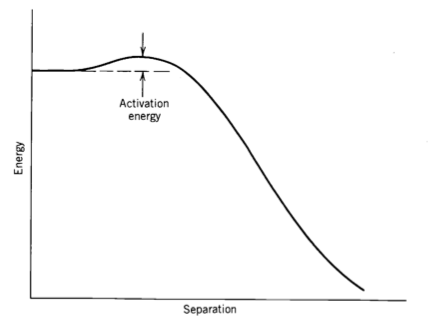
\includegraphics[scale=0.7]{smooth_fission_barrier.png}
 	\caption{The smooth fission barrier, illustrating the activation energy. Figure from K.S. Krane p.481 \cite{Krane1988}}
 	\label{fig:smooth_fission_barrier}
 \end{figure}

\noindent The energy released in fission is about the same as the activation energy needed to overcome the fission barrier. Those nuceli that have an energy release though fission that allows them to overcome most of the fission barrier, have a highter probability of tunnelling through the barrier \cite{Krane1988} (p.481). This is a known effect from quantum physics: the thinner the potential barrier, the larger the probability of tunnelling. These nuclei that see a thin potential barrier are thus called the spontaneously fissioning nuclei. However, most of the nuceli are not able to overcome much fission barrier by themselves, and thus they see a thick potential, and the probability of tunnelling is vanishing. They are therefore not unstable to spontaneous fission. This explains why the number of spontaneously fissioning nuclei are so few, even though it is energetically possible for plenty of the heavier nuclei to fission.

\par
\vspace{3mm}

\noindent This far I´ve only described the fission barrier using the liquid drop model. However, the liquid drop model is not a complete description of the nuclei, and shell effects have a impact when studying the probability to fission. When including the effects of the single particle shell structure, the fission barrier is changed to a barrier with two humps, called the double-humped fission barrier \cite{Krane1988} (p.495). The double-humped fission barrier is shown in Figure \ref{fig:double_humped_fission_barrier}. Nucei with energies well below the fission barrier , but above the well in the fission potential, thus sees two thinner barriers, compared to one thick barrier that the nuclei sees if it has energies below this well. They can tunnel through the first barrier, and then exist in an isomer state in the well, before either tunnelling through the second ponential hump, or gamma-decay back to the ground state.  The tunnelling of two thin barriers is more probable than tunnelling through one thick barrier, so the double-humped fission barrier makes more nuclei unstable to spontaneous fission. The existence of the double-humped fission barrier was confirmed when fission isomers were discovered, which are isotopes highly unstable to spontaneous fission \cite{Krane1988} (p.495). 

  \begin{figure}
 	\centering
 	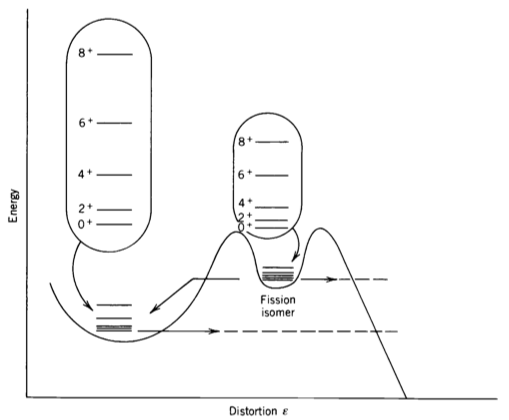
\includegraphics[scale=0.7]{double_humped_fission_barrier.png}
 	\caption{The double humped fission barrier Figure from K.S. Krane p.496 \cite{Krane1988}}
 	\label{fig:smooth_fission_barrier}
 \end{figure}

\noindent Even though states in the nucleus can have wave functions that have components in both the minimas of the double-humped fission barrier, the wave functions are usually are more prominent within one of the minimas. \cite{Wagemas1991}. It is therefore common to separate them into class I and class II states, where class I states are states concentrated in the first well, while class II states are concentrated in the second well. 

For some elements, the double humped fission barrier is further extended to a humtiple-humped fission barrier \cite{Goriely2017}. The triple-humped fission barrier have been observed for actinides, and for some reaction channels \cite{PhysRevC.74.014608}.
 
\subsection{The role of fission in nucleosynthesis}
In the beginning of the new milennia, a comitee of physicists and astronomers presentet what they ment was the 11 greatest, unanswered questions withing physics \cite{Haseltine2002}. One of these was how was the heavy elements in the universe, raging from iron to uranium, produced?

\par 
\vspace{3mm}
It has been known for some years that the light elements in the universe are produced through fusion of light elements into heavier elements. As seen from Figure \ref{fig:binding_energy_per_nucleon}, the average binding energy per nucleon increases up to about $A = 56$, and thus energy is released through fusion reactions. Iron, however, is the top of this curve. It is the bottom of the energy well, and energy can neither be released throug fission nor fusion We know, however, that elements up to uranium are produced somewhere in the universe, as we can observe them on Earth. This is why the comitee specified that the unanswered question is where the elements raging from iron to uranium are produced. 

\par
\vspace{3mm}

The physicist and astronomers are already underway of explaining the origin of plenty of the elements heavier than iron. The two, main processes often mentioned are the s-process and the r-process. Both are neutron capture processes. Iron can not fission nor fusion, but it can capture a neutron, and thus become unstable to $/beta$-decay. The s-process is the slow neutron-capture process, meaning that the frequency of neutron captures is low compared to the lifetimes of the nuclei created. It therefore only accounts for elements close to the valley of stability. The rapid neutron-capture process, however, consists of muntiple captures and decays, and can thus account for the production of far more unstable and heavier element than the s-process. Thus, the r-process needs a much higher neutron flux to occur, compared to the s-process. Through the s- and r-processes, and several more processes, one are beginning to see the outline of the isotope composition of the universe. Still, there is a long way to go before one of the greatm unanswered questions in physics can be ticked off the list.

\par 
\vspace{3mm}

As mentioned above, the r-process produces heavy, neutron-rich nuclei. These are often thought of to $\beta$-decay back to the valley of stability, but this is by far not the only possible reaction channel they can undergo. These nuclei can also undergo fission, and then produce several new, lighter nuclei.

Fission is usually though of maybe being the production reaction for light nuclei, in the interval A$\approx 110 - 160$, because the way new elements would be produced would be as the fission product of a heavy, neutron rich nucleus. If the fission fragments still is located in an area with high neutron flux, the fission fragments will continue to absorb neutrons, again becoming heavy nuclei, which can fission again. This process is known as fission recycling \cite{Goriely2017}. When the neutron flux decreases, the recyclin process will stop, leaving the fission fragments to decay towards stability. Fission in the nucelosynthesis is not solely neutron induces, it can be spontaneous or $/beta$-delayed, and also gamma induced, the latter often referred to as photofission \cite{Goriely2017}. 

\par 
\vspace{3mm}

When determining if we have understood the nucleosynthesis, we rely on simultions of the procuction of the elements, comparing it to the element distrubution we can observe in the universe today.  The challenge when determining the fission's role in the synthesis of heavy elements, is that there are plenty of nuclear properties needed as input to these simulations, half-lives, reaction channel cross sections and fission barriers to mention some. Not only are these properties not always measured for all elements that can be produced in the laberatory, but one also need these properties for exotic nuclei, far from the valley of stability. Predictions must then be used for describing these exotic nuclei's properties, making the simulations of the fission's role in nucleosynthesis unreliable and heavily model dependent. 



\section{Method}

\subsection{TALYS}

TALYS is a computer code for computing reaction cross sections for nuclear reactions \cite{TALYSmanual}, and it is a handy tool for predicting outcomes of experiments before conducting them. TALYS can simulate light incident particles for a wide range of energies, hitting nuclei in the atomic mass region $12<A>339$ \cite{TALYSmanual}. The code will then provide the cross sections for different reactions to occur. The code is also highly customizable. It will provide a set of default values and models that can easily changed to study the impact of different models on the reaction cross sections.

\subsection{(n,$\gamma$) and (n,f) cross sections sensitivity to changes in the fission barrier of $\ce{^{240}Pu}$}

In all experimental sciences, one must accept that we only know certain parameters within a given uncertainty, and experimental nuclear physics is no different. Parameters such as mass, level density and excitation energy is not known as an absolute value. This, however, is bothersome when trying to conduct simulations where these values are needed as input. The simulation will be no better than the uncertainty of the nuclear values it sorely needs as input parameters. If the simulation additionally is extremely dependent on the values of this imput, the output of the simulation can yield vastly different answers for a slight variation in one of the input variables. It is therefore important to be aware of such dependences when conducting simulations. 

\par 
\vspace{3mm}

In this report, I will test the sensitivity of the (n, $\gamma$) and (n,f) cross sections for $\ce{^{240}Pu}$ upon changes in the fission barrier, to determine wheter or not TALYS might be likely to predict these cross sections correctly before my master experiment runs in April 2018.

\par 
\vspace{3mm}

My master experiment is the (d,p)-induced fission of $\ce{^{240}Pu}$, and it is used as the surrogate reaction of (n,f), assuming that the incoming reaction channel does not affect the reaction cross sections. I will thus calculate the cross sections for $\ce{^{240}Pu}$(n,f) with TALYS. The incoming deuteron energy used in the experiment will be $\approx$ 12 MeV, but the proton will carry some of this kinetic energy away from the nucleus. Thus we expect the neutron to bring up to 4 MeV (?) to the nuclei, and therefore I will use neutron energies up to 4 MeV in this simulation. 
\par 
\vspace{3mm}

I will first calculate the cross sections using the default fission barrier values in TALYS, and then change the fission barrier and observe the changes happening in the reaction cross sections.

\section{Results}

\section{Discussion}

\section{Conclusion}


\bibliographystyle{plain}
\bibliography{TALYS.bib} 






\end{document}
